\subsection{Setup 1 - KMeans: Resultados nos Datasets Adult e Dry Bean}

Neste primeiro setup, avaliamos o desempenho do KMeans supervisionado nos conjuntos Adult (balanceado) e Dry Bean (balanceado), ambos após pré-processamento e balanceamento por oversampling. O pipeline seguiu rigorosamente as etapas de normalização, divisão estratificada, definição do número de clusters, treinamento, repetição dos experimentos (30 execuções) e análise quantitativa detalhada.

\subsubsection{Adult (Balanceado)}

O KMeans foi executado com $n_{clusters}=8$. Os resultados médios das 30 repetições estão na Tabela~\ref{tab:kmeans_adult_metrics}. O desempenho foi avaliado por métricas macro e matriz de confusão média. Observa-se que o balanceamento das classes foi fundamental para evitar viés para as classes majoritárias, permitindo uma avaliação mais justa do agrupamento.

% Tabela Adult apenas acurácia e desvio padrão
\begin{table}[H]
\centering
\caption{Resultados quantitativos do KMeans no dataset Adult (balanceado, $n_{clusters}=8$)}
\label{tab:kmeans_adult_metrics}
\begin{tabular}{lcc}
\toprule
Métrica & Média & Desvio Padrão \\
\midrule
Acurácia & 0.7117 & 0.2883 \\
\bottomrule
\end{tabular}
\end{table}


A matriz de confusão média está ilustrada na Figura~\ref{fig:kmeans_adult_balance_confusion_matrix_media}:
\begin{figure}[ht]
    \centering
    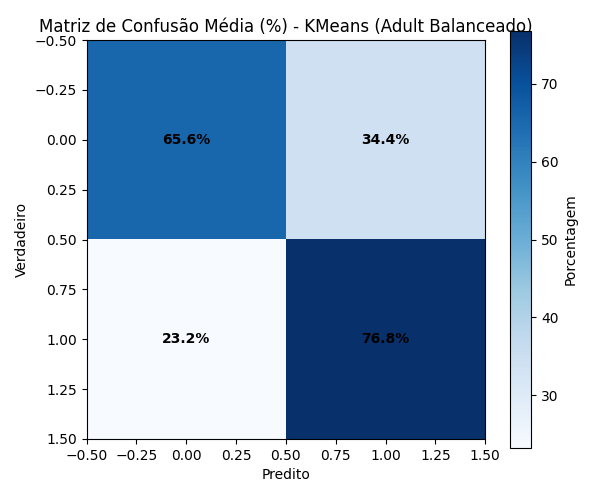
\includegraphics[width=0.7\linewidth]{../src/img/kmeans_adult_balance_confusion_matrix_media_percent.png}
    \caption{Matriz de confusão média (KMeans - Adult Balanceado)}
    \label{fig:kmeans_adult_balance_confusion_matrix_media}
\end{figure}

As principais visualizações estão apresentadas a seguir:
\begin{figure}[ht]
    \centering
    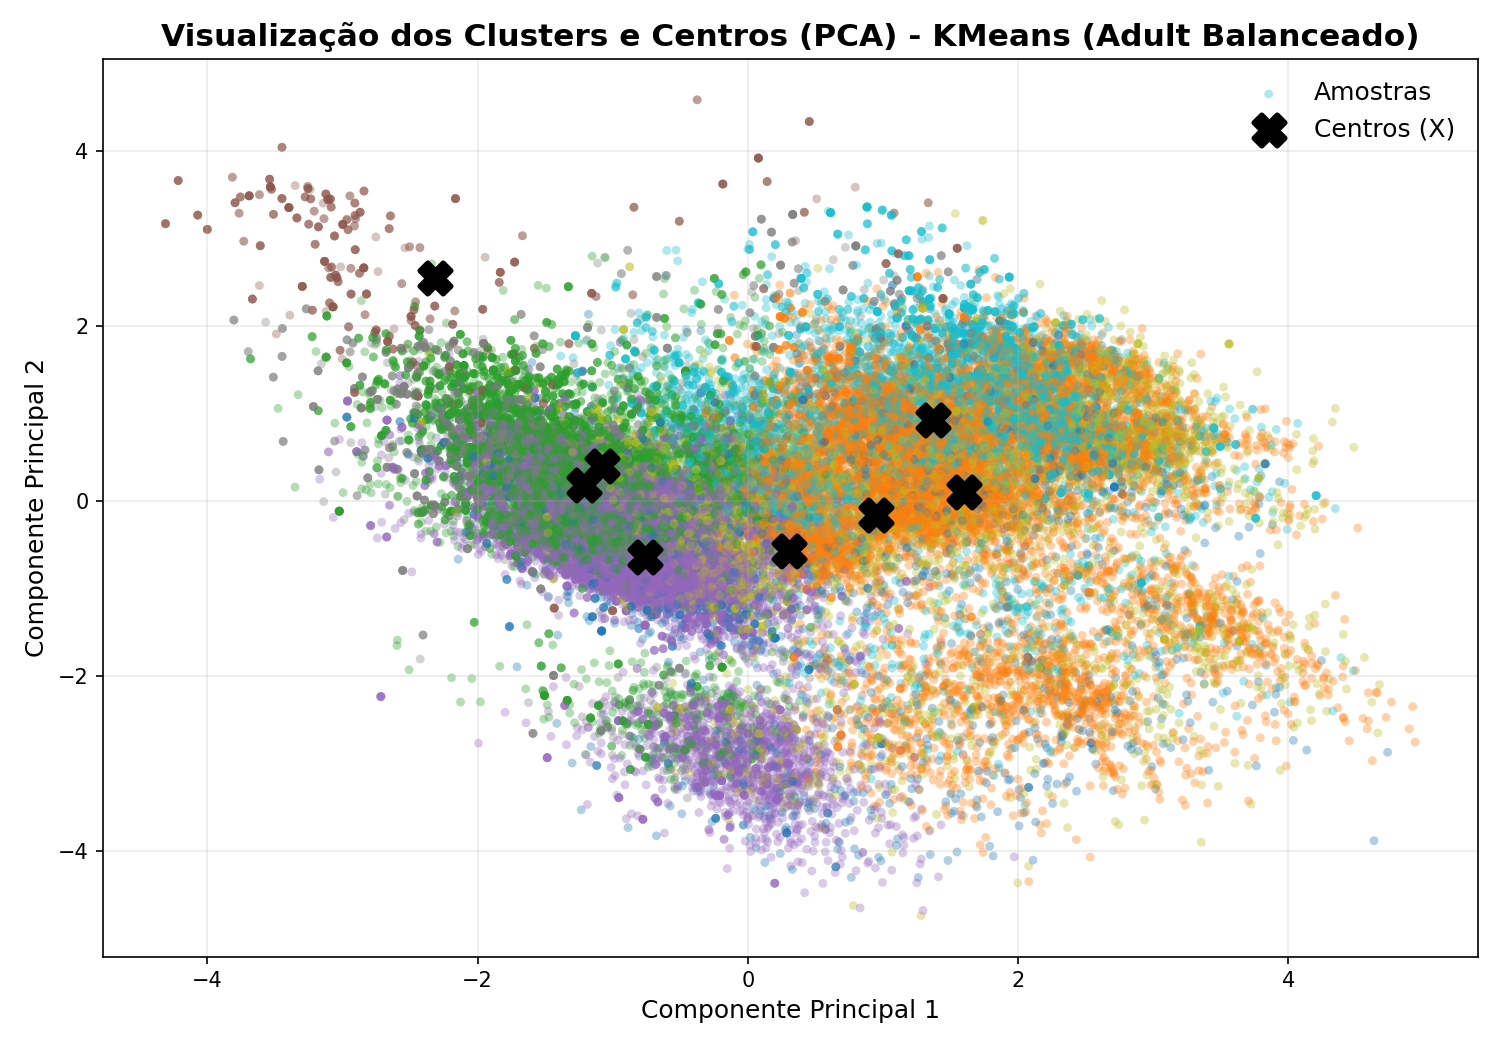
\includegraphics[width=0.7\linewidth]{../src/img/kmeans_adult_balance_clusters_pca.png}
    \caption{Visualização PCA dos clusters e centros (KMeans - Adult Balanceado)}
    \label{fig:kmeans_adult_pca}
\end{figure}
\begin{figure}[ht]
    \centering
    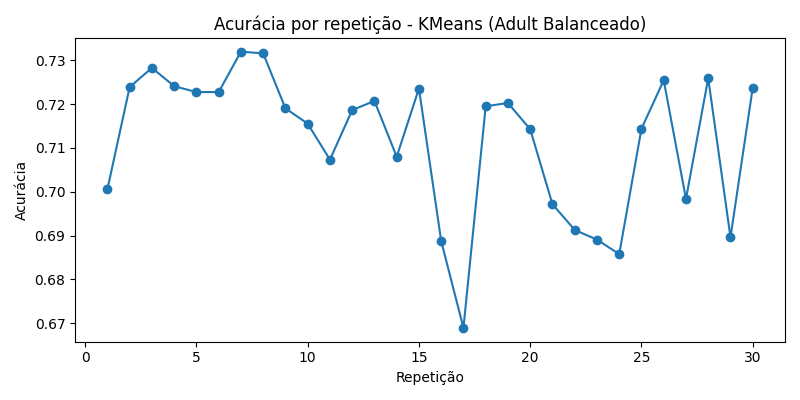
\includegraphics[width=0.7\linewidth]{../src/img/kmeans_adult_balance_accuracy_repetitions.png}
    \caption{Acurácia por repetição (KMeans - Adult Balanceado)}
\end{figure}
\begin{figure}[ht]
    \centering
    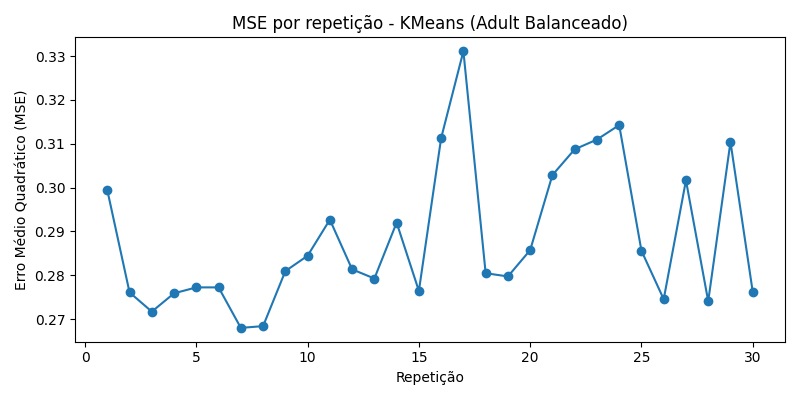
\includegraphics[width=0.7\linewidth]{../src/img/kmeans_adult_balance_mse_repetitions.png}
    \caption{MSE por repetição (KMeans - Adult Balanceado)}
\end{figure}


\subsubsection{Dry Bean (Balanceado)}

No dataset Dry Bean, o KMeans também foi executado com $n_{clusters}=7$ e 30 repetições. Os resultados estão sumarizados na Tabela~\ref{tab:kmeans_drybean_metrics}. O desempenho foi superior ao observado no Adult, refletindo a maior separabilidade das classes neste conjunto multiclasse.

% Tabela Dry Bean apenas acurácia e desvio padrão
\begin{table}[H]
\centering
\caption{Resultados quantitativos do KMeans no dataset Dry Bean (balanceado, $n_{clusters}=7$)}
\label{tab:kmeans_drybean_metrics}
\begin{tabular}{lcc}
\toprule
Métrica & Média & Desvio Padrão \\
\midrule
Acurácia & 0.7537 & 0.2840 \\
\bottomrule
\end{tabular}
\end{table}


A matriz de confusão média está ilustrada na Figura~\ref{fig:kmeans_drybean_balance_confusion_matrix_media}:
\begin{figure}[ht]
    \centering
    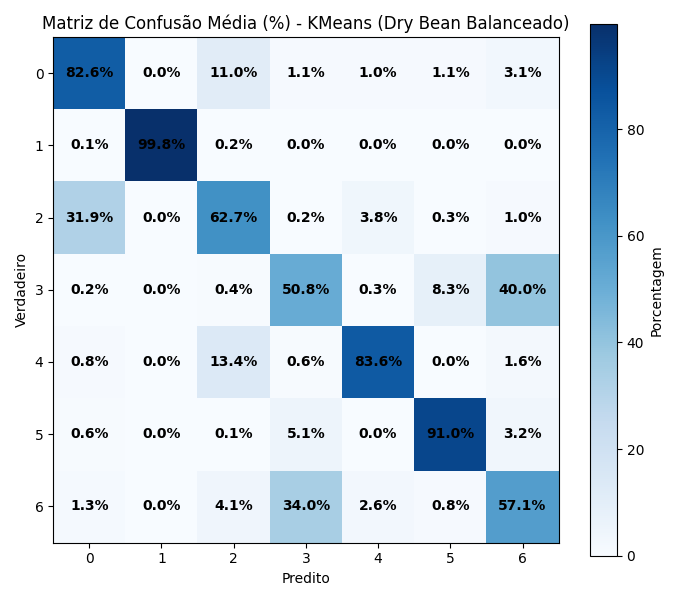
\includegraphics[width=0.7\linewidth]{../src/img/kmeans_drybean_balance_confusion_matrix_media_percent.png}
    \caption{Matriz de confusão média (KMeans - Dry Bean Balanceado)}
    \label{fig:kmeans_drybean_balance_confusion_matrix_media}
\end{figure}

As principais visualizações estão apresentadas a seguir:
\begin{figure}[ht]
    \centering
    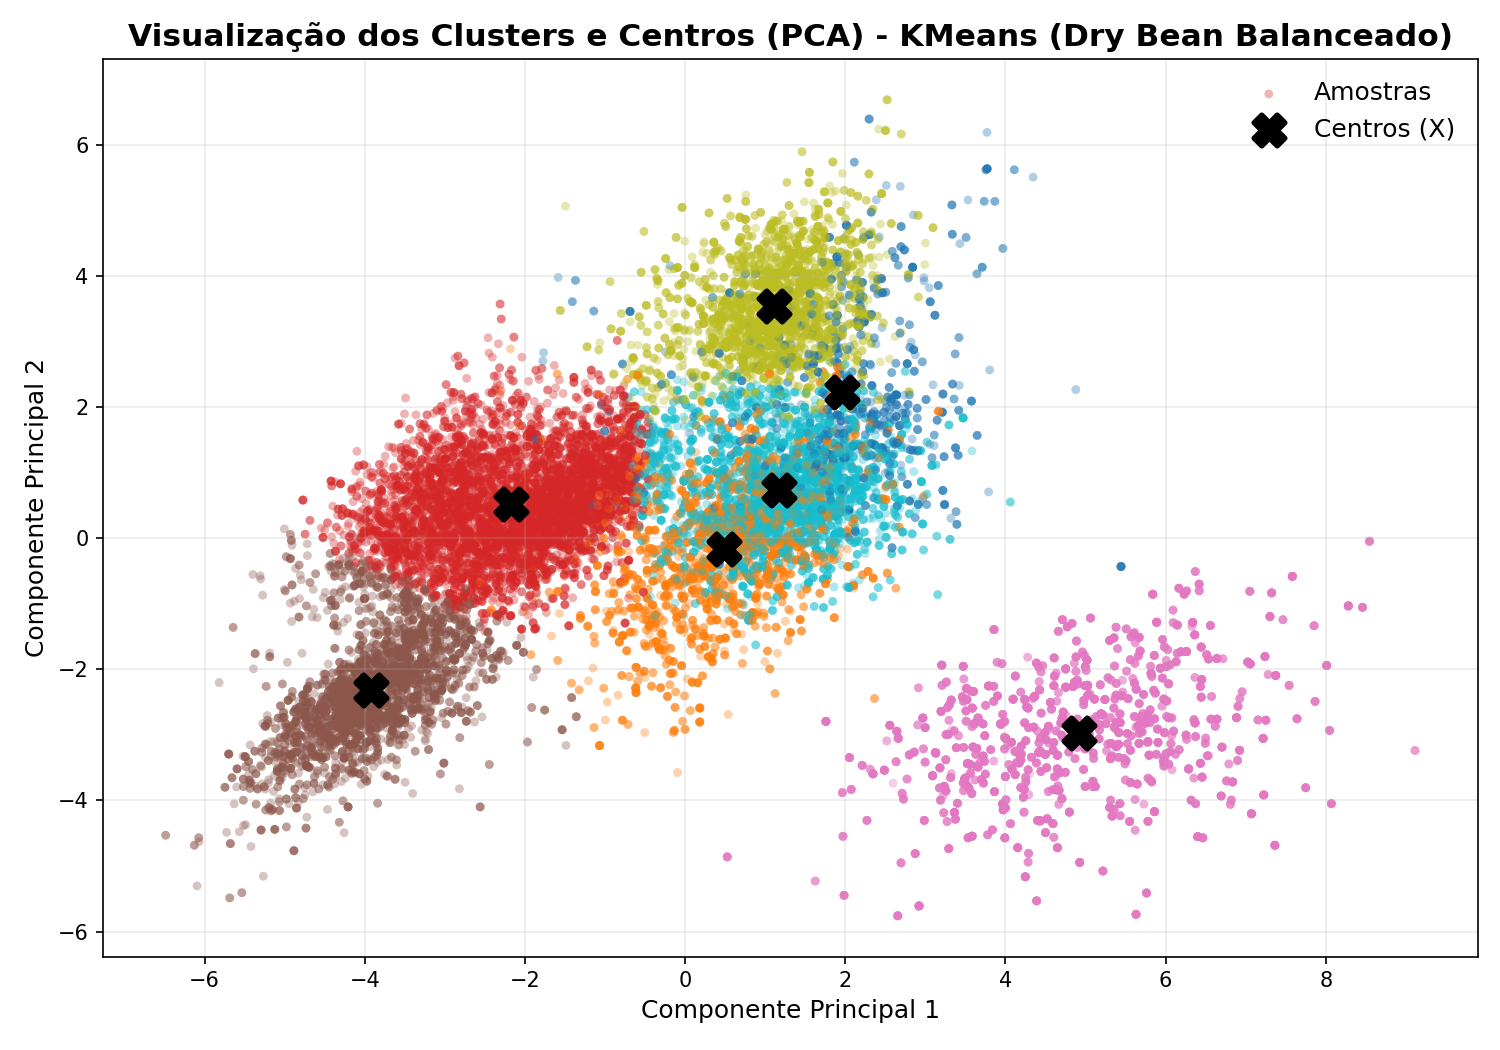
\includegraphics[width=0.7\linewidth]{../src/img/kmeans_drybean_balance_clusters_pca.png}
    \caption{Visualização PCA dos clusters e centros (KMeans - Dry Bean Balanceado)}
\end{figure}
\begin{figure}[ht]
    \centering
    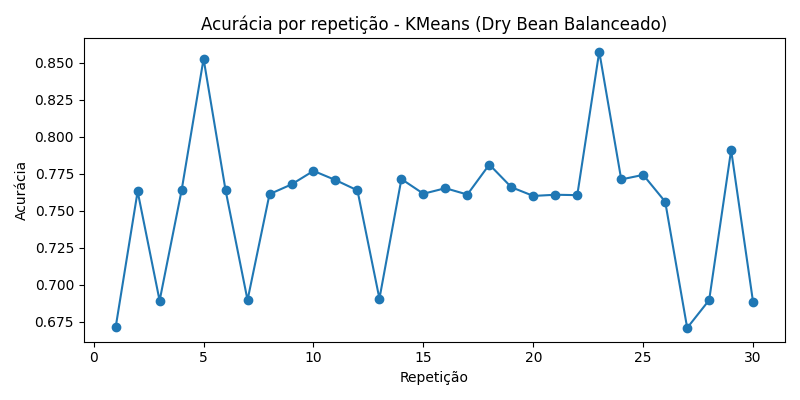
\includegraphics[width=0.7\linewidth]{../src/img/kmeans_drybean_balance_accuracy_repetitions.png}
    \caption{Acurácia por repetição (KMeans - Dry Bean Balanceado)}
\end{figure}
\begin{figure}[ht]
    \centering
    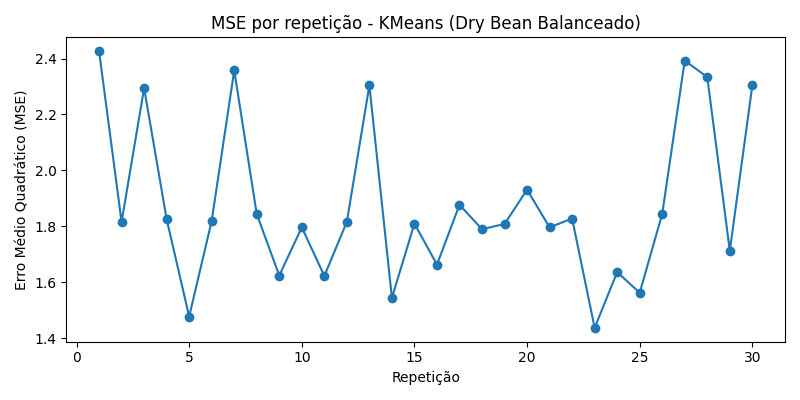
\includegraphics[width=0.7\linewidth]{../src/img/kmeans_drybean_balance_mse_repetitions.png}
    \caption{MSE por repetição (KMeans - Dry Bean Balanceado)}
\end{figure}

